\documentclass[12pt,twoside]{article} 
\usepackage{amsmath, amssymb} 
\usepackage{graphicx}
\usepackage{amsmath} 
\usepackage[active]{srcltx} 
\usepackage{amssymb} 
\usepackage{amscd} 
\usepackage{makeidx} 
\usepackage{amsthm} 
\usepackage{algpseudocode} 
\usepackage{algorithm}
\usepackage[spanish, activeacute]{babel}
\usepackage[utf8]{inputenc}

\renewcommand{\baselinestretch}{1}
\setcounter{page}{1}
\setlength{\textheight}{21.6cm}
\setlength{\textwidth}{14cm}
\setlength{\oddsidemargin}{1cm}
\setlength{\evensidemargin}{1cm}
\pagestyle{myheadings}
\thispagestyle{empty}
\markboth{\small{Pr\'actica 4. Fernando Rivera, Alejandro Contreras}}{\small{.}}

\begin{document}
\centerline{\bf An\'alisis de Algoritmos, Sem: 2020-1, 3CV2, Pr\'actica 4}
\centerline{}
\centerline{11 - 09 - 2019}
\begin{center}
\Large{\textsc{Pr\'actica 4: Divide y vencerás parte II}}
\end{center}
\centerline{}
\centerline{\bf {Rivera Paredes Fernando Daniel, Contreras Paredes Alejandro.}}
\centerline{}
\centerline{Escuela Superior de C\'omputo}
\centerline{Instituto Polit\'ecnico Nacional, M\'exico}
\centerline{$ferny036@hotmail.com, acontrerasparedes@hotmail.com$}
\newtheorem{Theorem}{\quad Theorem}[section] \newtheorem{Definition}[Theorem]{\quad Definition} \newtheorem{Corollary}[Theorem]{\quad Corollary} \newtheorem{Lemma}[Theorem]{\quad Lemma} \newtheorem{Example}[Theorem]{\quad Example} \bigskip
\textbf{Resumen:} Nuevamente, retomamos la idea acerca de la metodología de divide y vencerás implementado en los distintos algoritmos, en este caso, un nuevo algoritmo de 
ordenamiento llamado \textbf{QuickSort}, el cual, se apoya con otro algoritmo llamado \textbf{Partition} para hacer la partición del arreglo y poder ordenarlos en su mínima expresión.

\centerline{}
{\bf Palabras Clave:} Divide, Vencerás, Logarítmico, QuickSort, Gráfica
\newpage

\section{Introducción}
Para la siguiente practica se hizo uso del conocimiento obtenido de la recursividad de funciones y la relaci\'on de una con otra se buscara implentar y ver la complejidad 
de los algoritmos merge y merge-sort. como antecedentes tenemos el ´´divide y venceras'' el cual se aplica cuando un problema se resuelve de forma recursiva
de tal manera que el problema principal se descompone en subproblemas del mismo tipo para encontrar un caso base para posteriormente resolverlos y juntarlo para tener soluci\'on del problema orinal


\section{Conceptos B\'asicos} 
\subsection{\textbf{Divide y vencerás}}
\setlength{\parindent}{1.5em}El término Divide y Vencerás en su acepción más amplia es algo más que una técnica de diseño de algoritmos. De hecho, suele ser considerada una filosofía general para resolver problemas y de aquí que su nombre no sólo forme parte del vocabulario informático, sino que también se utiliza en muchos otros ámbitos.
En nuestro contexto, Divide y Vencerás es una técnica de diseño de algoritmos que consiste en resolver un problema a partir de la solución de subproblemas del mismo tipo, pero de menor tamaño. Si los subproblemas son todavía relativamente grandes se aplicará de nuevo esta técnica hasta alcanzar subproblemas lo suficientemente pequeños para ser solucionados directamente. Ello naturalmente sugiere el uso de la recursión en las implementaciones de estos algoritmos.
La resolución de un problema mediante esta técnica consta fundamentalmente de los siguientes pasos:
\begin{enumerate}
  \item En primer lugar ha de plantearse el problema de forma que pueda ser descompuesto en k subproblemas del mismo tipo, pero de menor tamaño. Es decir, si el tamaño de la entrada es n, hemos de conseguir dividir el problema en k subproblemas (donde 1 ≤ k ≤ n), cada uno con una entrada de tamaño nk y donde 0 ≤ nk < n. A esta tarea se le conoce como división.
  \item En segundo lugar han de resolverse independientemente todos los subproblemas, bien directamente si son elementales o bien de forma recursiva. El hecho de que el tamaño de los subproblemas sea estrictamente menor que el tamaño original del problema nos garantiza la convergencia hacia los casos elementales, también denominados casos base.
  \item Por último, combinar las soluciones obtenidas en el paso anterior para construir la solución del problema original.
\end{enumerate}
\centerline{}


\section{Experimentaci\'on y Resultados}
\subsection{\textbf{Planteamiento de los distintos problemas}}
En el desarrollo de la práctica hay que demostrar varios puntos, los cuales son: 
\begin{enumerate}
  \item Demostrar que el algoritmo \textbf{Partition} tiene complejidad lineal.
  \item Demostrar que el algoritmo \textbf{QuickSort} tiene complejidad $\Theta (n \log (n))$.
  \item Encontrar los peores casos para el Algotimo de \textbf{QuickSort}, y cual es su complejidad.
\end{enumerate}
\centerline{}
\subsection{\textbf{Solución al primer problema}}

Para el desarrollo del algoritmo de \textit{Partition} se propuso el \textbf{Algoritmo 1}

\begin{algorithm}
  \caption{Partition}\label{euclid}
  \begin{algorithmic}[1]
  \Function{Partition}{$A[0, ..., n-1], p, r$}
      \State $x \gets A[r]$ \Comment $O(1)$
      \State $i\gets p - 1$ \Comment $O(1)$
      \For{$j = p$ \textbf{to} $j < r$} \Comment $O(n)$
        \If{$A[j] \leq x$} \Comment $O(1)$
          \State $i \gets i + 1$ \Comment $O(1)$
          \State $aux \gets A[i]$ \Comment $O(1)$
          \State $A[i] \gets A[j]$ \Comment $O(1)$
          \State $A[j] \gets aux$ \Comment $O(1)$
        \EndIf
        \State $j \gets j + 1$ \Comment $O(1)$
      \EndFor
      \State $aux \gets A[i+1]$ \Comment $O(1)$
      \State $A[i+1] \gets A[r]$ \Comment $O(1)$
      \State $A[r] \gets aux$ \Comment $O(1)$
      \State \textbf{return} $i + 1$ \Comment $O(1)$
  \EndFunction
  \end{algorithmic}
\end{algorithm}

La cual para verificar analíticamente su grado de complejidad de acuerdo a los comentarios, de una manera simplificada lo podemos ver de la siguiente
manera: 

\centerline{$T(n) = 2*O(1)+O(n)[7*O(1)]+4*O(1)$}
\centerline{}
\centerline{donde: $O(g(n))_{1} + O(g(n))_{2}+\cdots+O(g(n))_n = O(g(n))$}
\centerline{}
\centerline{$\Rightarrow T(n) = O(1)+O(n)[O(1)]$}
\centerline{}
\centerline{donde: $O(f(n)) * O(g(n))= O(f(n)*g(n))$}
\centerline{}
\centerline{$\Rightarrow T(n) = O(1) + O(n)$}
\centerline{}
\centerline{donde: $O(f(n)) + O(g(n)) = O(h(n))$}
\centerline{y $h(n)$ es la funci\'on con mayor jeraqu\'ia respecto a $g(n)$ y $f(n)$}
\centerline{}
\centerline{$\therefore T(n) \in O(n)$}

Podemos notar en $Figure$ $1$ el comportamiento del algoritmo \textbf{Partition}, con linea punteada se puede visualizar el caso cuando todos los 
elementos del arreglo son iguales. Concluyendo que seria el peor de los casos de manera lineal.
\begin{figure}
  \centering
    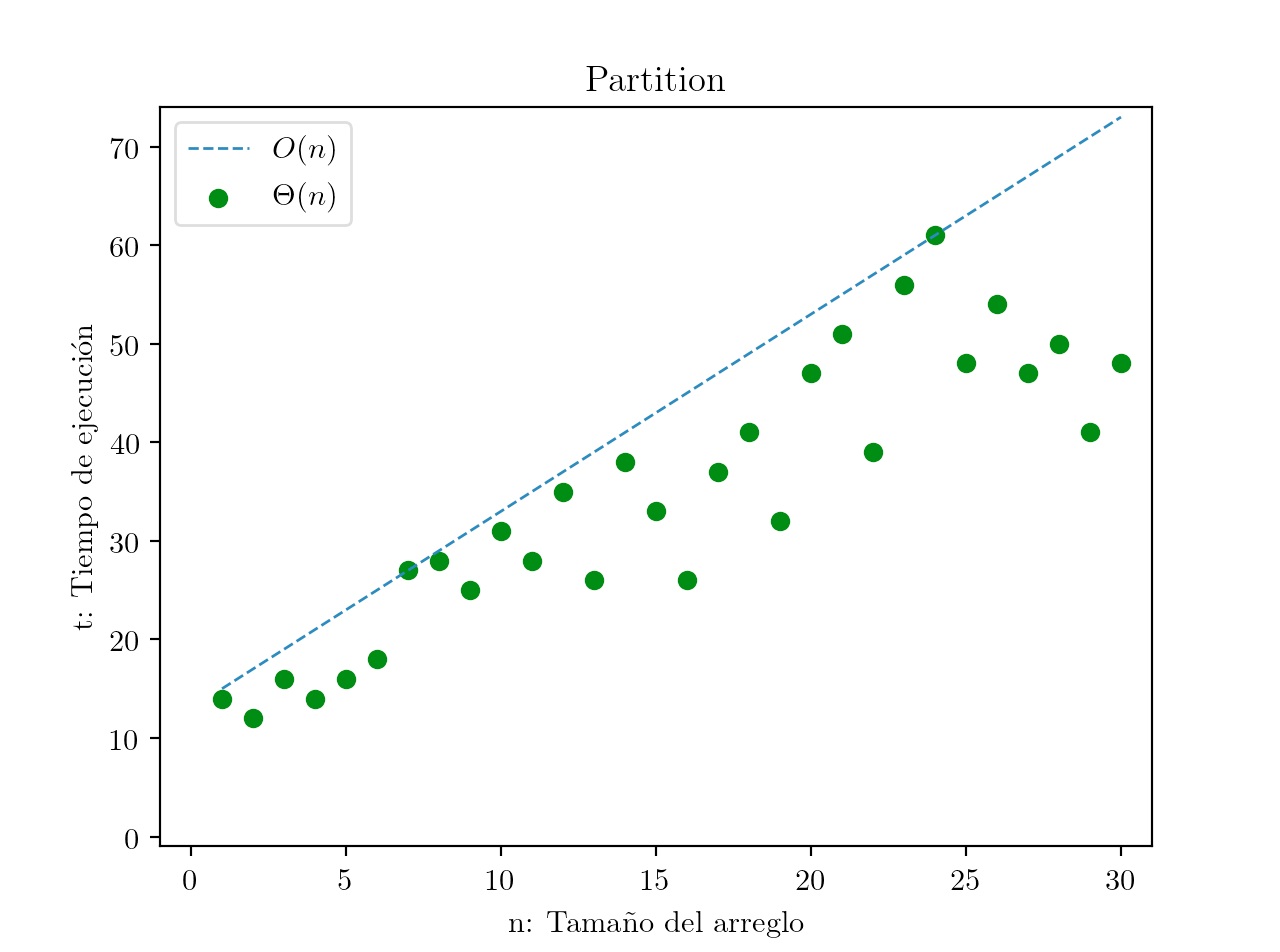
\includegraphics[height=0.5\textwidth]{Figure1}
  \caption{Comportamiento del algoritmo Partition}
  \label{fig:ejemplo1}
\end{figure}

\subsection{\textbf{Soluci\'on al segundo problema}}

Para el desarrollo del algoritmo de \textbf{QuickSort} hay que hacer un uso del algoritmo \textbf{Partition} anteriormente resuelto; dónde éste
determina el pivote de nuestro arreglo a ordenar, y aqui es donde entra \textbf{QuickSort}, tanto que de manera recursiva, va determinando con 
\textbf{Partition}, los distintos pivotes de cada uno de los subarreglos y ordenarlos. Donde el algoritmo a proponer sería el \textbf{Algoritmo 2}.


\begin{algorithm}
  \caption{QuickSort}
  \begin{algorithmic}[1]
  \Function{QuickSort}{$A[0, ..., n-1], p, r$}
    \If{$p<r$} \Comment $O(1)$
      \State $q \gets Partition(A, p, r)$ \Comment $O(n)$
      \State $QuickSort(A,p,q)$ \Comment $T(p - q)$
      \State $QuickSort(A,q + 1,r)$ \Comment $T(r - q + 1)$
    \EndIf
  \EndFunction
  \end{algorithmic}
\end{algorithm}

De acuerdo al análisis anterior del algoritmo de \textit{Partition} concluimos que tiene complejidad $O(n)$, entonces, para poder analizar 
el comportamiento del algoritmo de \textit{QuickSort}, creamos su función de recurrencia, tomando en cuenta la relación de acuerdo a qué términos
juegan el papel del término $n$, entonces, a esta relación se le atribuye $n = r - p$. Considerando que el pivote siempre se elije por la mitad del
arreglo, se puede decir que:
\centerline{}
\centerline{$r - q = q - p = \frac{n}{2}$}
\centerline{$\therefore T(p - q) = T(r - q + 1) = T(\frac{n}{2})$}

Entonces, creamos nuestra ecuación de recurrencia con estas propiedades de tal manera que cumpla los valores anteriores:
\begin{center}
  $T(n) =\left\{ \begin{array}{lcc}
      c_{1} &   si& n=1\\
  \\  2*T(\frac{n}{2}) + c_{2}*n &  si  & n>1 
  \end{array}
  \right.
  $
\end{center}

Debido a que no tenemos nocion acerca de $T(\frac{n}{2})$, optaremos por construir una nueva función de recurrencia a partir 
de la transformación $n = \log_{2} k \Rightarrow k = 2^n$. Entonces $T(n)$ en términos de $k$ sería:

\begin{center}
  $T(2^k) =\left\{ \begin{array}{lcc}
      c &   si& k=0\\
  \\  2*T(2^{k-1}) + c*2^k &  si  & k>0 
  \end{array}
  \right.
  $
\end{center}

Se tiene:\\

  $T(2^k)=2*T(2^{k-1}) + c*2^k$\\
  $T(2^k)=2*[2*T(2^{k-2}) + c*2^{k-1}] + c*2^k$\\
  $T(2^k)=2^2*T(2^{k-2}) + 2*c*2^k$\\
  $T(2^k)=2^2*[2*T(2^{k-3}) + c*2^{k-2}] + 2*c*2^k$\\
  $T(2^k)=2^3*T(2^{k-3}) + 3*c*2^k$\\
  $\vdots$\\
  $T(2^k)=2^i*T(2^{k-i}) + i*c*2^k$\\ 
  \centerline{}
  Si $k = i$, entonces:\\
  $T(2^k)=2^k*T(1) + k*c*2^k$\\ 
  \centerline{}
  Regresando a $n$:\\
  $T(n)=n*T(1) + \log_{2}(n)*c*n$\\
  $\therefore T(n) \in O(n \log(n))$\\ \\

Recordemos que este es el grado de compleidad para \textbf{QuickSort} cuando la función \textbf{Partition} divide a la mitad el arreglo. 

\subsection{\textbf{Soluci\'on al tercer problema}}
Ahora nos preguntamos que sucede si el pivote se elige de otra manera que no sea completamente por la mitad, asi que se propone ejecutar el
algoritmo de \textbf{QuickSort} con la lista ordenada de una manera decreciente, o bien, tambien puede ser que la lista tenga el mismo elemento,
en valor, en cada una de las posiciones del arreglo, tomaremos el primer caso y ejecutandolo nos lanza la gráfica de la figura 2.

\begin{figure}
  \centering
    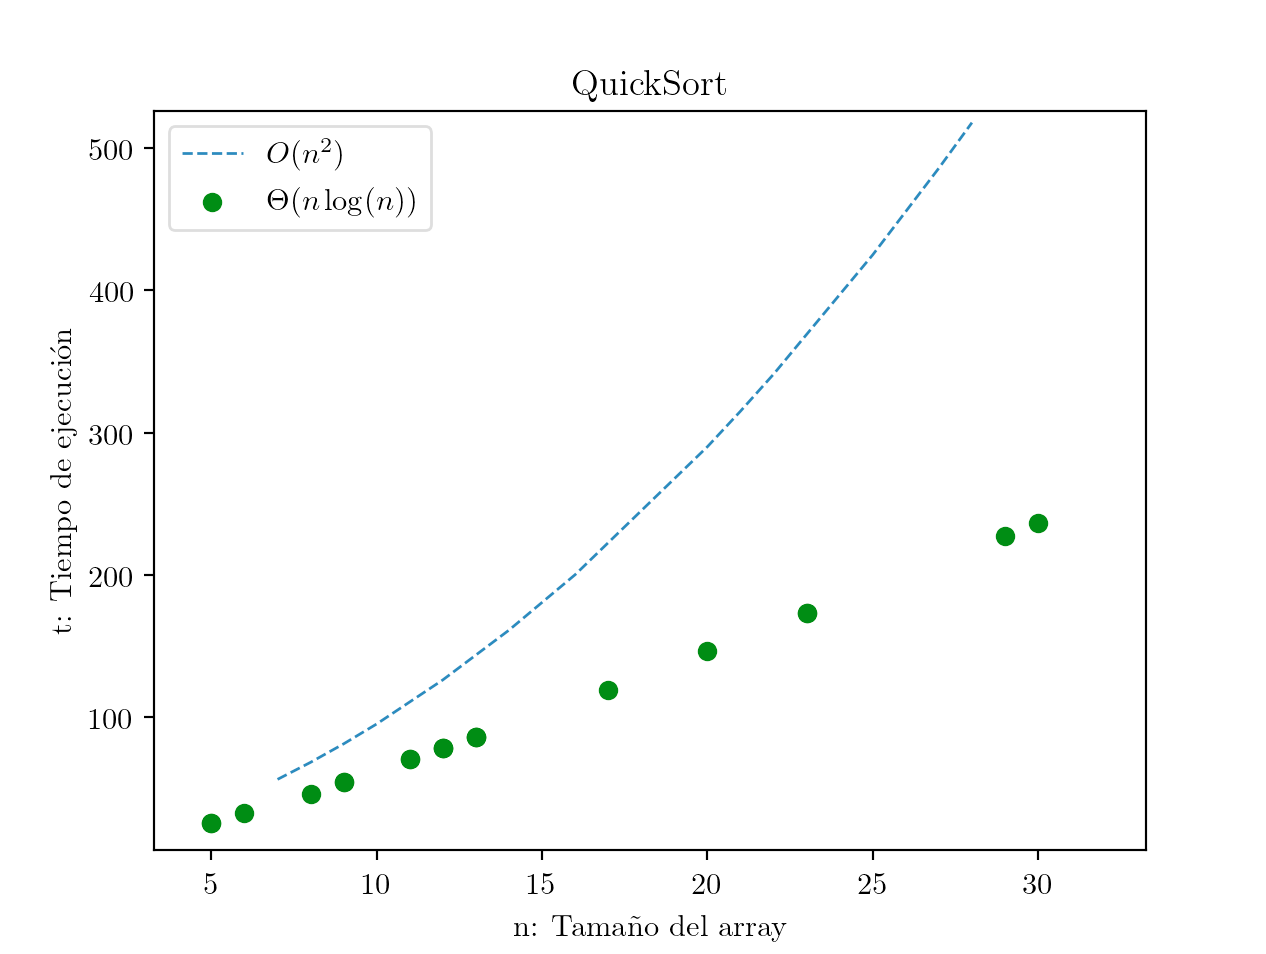
\includegraphics[height=0.5\textwidth]{Figure2}
  \caption{Comportamiento de QuickSort}
  \label{fig:ejemplo3}
\end{figure}

Con lo que podemos concluir de acuerdo a la gráfica que cuando los elementos son iguales o estan ordenados de manera descendiente, nos genera una
función cuadrática($O(n^2)$), a comparación que si elegimos siempre la mitad del arreglo, lo cual nos produce una complejidad de $n \log(n)$ $Figure$ $2$.
\newpage

\section{Anexo} 
\text{}\\ 
\textbf{Preguntas}
\begin{enumerate}
  \item ¿Qué valor de q retorna \textbf{Partition} cuando todos los elementos en el arreglo $A[p, ..., r]$ tienen el mismo valor?.\\\\
    \textbf{R.} El valor que retorna de $q$ al ejecutar el algoritmo \textbf{Partition} cuando todos los elementos son iguales siempre es
    $r$, y esto es facil de determinar, debido a que, en la condición del $if$ no pide que sea estrictamente menor, por lo que el índice
    $i$ siempre incrementa hasta llegar a la posición $r - 1$, dónde se realiza el último cambio y posteriormente, retorna el valor de $r$. 
  \item ¿Cuál es el tiempo de ejecución de \textbf{QuickSort} cuando todos los elementos del arreglo tienen el mismo valor?.\\\\
  \textbf{R.} El tiempo de ejecución del algoritmo \textbf{QuickSort}(complejidad) cuando todos sus elementos tienen el mismo valor, es el mismo
  el cual a la solución del tercer problema planteado anteriormente, solo que en éste punto el pivote que se elige siempre es el último elemento
  lo cual produce que tenga una complejidad similar al tercer problema de $O(n^2)$ 
\end{enumerate}

\newpage
\section{Conclusiones}
\textbf{Conclusion Alejandro Contreras Paredes}\\
Para el desarrollo de esta practica usamos los algoritmos que fueron desarollados en clase, de los cuales, uno estaba incompleto
lo que represento un problema a la hora de la codificación, esto represento un pequeño retraso pero finalmente pudimos solucionarlo. Por otra
parte, esta practica reafirma la teoria de la complejidad de los algoritmos recursivos y finalmente las graficas fueron realizadas conforme a las indicaciones
especificadas.\\\\
\textbf{Conclusion Fernando Daniel Rivera Paredes}\\

En el desarrollo de la práctica, tuvimos un primer percance respecto al algoritmo de Merge, debido a que esta incompleto, y faltaba un manejo
correcto de los indices al desbordamiento de los índices, estuvo muy bien el manejo ante esa "trampa`` en el código, para que uno como alumno
autodidacta pretenda realizar una solución sin afectar la complejidad del algoritmo. Finalmente, la parte gráfica solía ser muy confusa al inicio
dado que no se podía visualizar correctamente las curvas que mostraban. 
\begin{figure}[!h]
	\centering
	\begin{minipage}[t]{10cm}
		\centering
		
\includegraphics[scale=0.2]{Foto1}
		\caption{Alejandro Contreras Paredes}
	\end{minipage}
	\hspace{18cm}
	\begin{minipage}[t]{10cm}
		\centering
		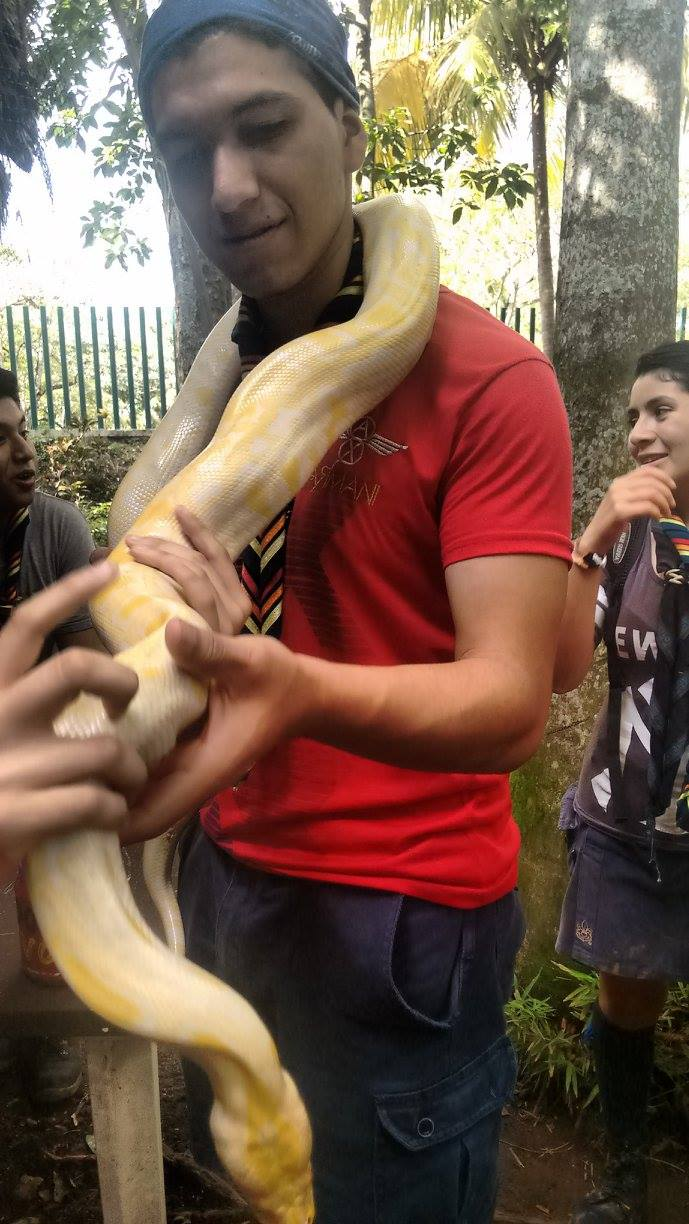
\includegraphics[scale=0.2]{Foto2}
		\caption{Rivera Paredes Fernando Daniel}
	\end{minipage}
\end{figure}

\section{Bibliograf\'ia}

\begin{thebibliography}{9}
  \bibitem{book} 
  Cormen, T. and Leiserson, C.
  \textit{Introduction to algorithms.} 
  3rd edition.Cambridge, Massachusetts: Massachusetts Institute of Technology, 2009.

  \bibitem{ie} 
  Moyano, N.
  \textit{Análisis de algoritmos}.
  Medium. Available at: $www.lcc.uma.es/~av/Libro/CAP3.pdf$'[Accessed 03 Sep. 2019].
\end{thebibliography}
\end{document}
